\documentclass[runningheads]{llncs}

\usepackage[mobile]{eccv}


% ---------------------------------------------------------------
% packages

% Commonly used abbreviations (\eg, \ie, \etc, \cf, \etal, etc.)
\usepackage{eccvabbrv}

\usepackage{preamble}

\usepackage[accsupp]{axessibility}  % Improves PDF readability for those with disabilities.


\usepackage[pagebackref,breaklinks,colorlinks,citecolor=eccvblue]{hyperref}

\usepackage{enumitem}
%\usepackage{tocloft}

\begin{document}
	
	% ---------------------------------------------------------------
	\title{Efficient Transformer Encoders for Mask2Former-style models} 
	
	% an abbreviated paper title here. If not, comment out.
	\titlerunning{Efficient Transformer Encoders for Mask2Former-style models}
	
	\author{Manyi Yao\inst{2} \and
		Abhishek Aich\inst{1} \and
		Yumin Suh\inst{1} \and Amit Roy-Chowdhury\inst{2} \and \\Christian Shelton\inst{2}\and Manmohan Chandraker\inst{1,3} }
	
	\authorrunning{M.~Yao et al.}
	
	\institute{NEC Laboratories, America, San Jose CA 95110, USA 
		\and
		University of California, Riverside, CA 92521, USA
		\and
		University of California, San Diego, CA 92093, USA\\
		Corresponding author: \email{aaich@nec-labs.com} 
	}
	
	\maketitle
	%\hypersetup{
		%    linkcolor=eccvblue,  % color of internal links 
		%    citecolor=eccvblue,  % color of links to bibliography
		%}
	\FloatBarrier
	\sloppy
	
	
	% \setlength{\textfloatsep}{0.5cm}
	% -------- Abstract -------- %
	\begin{abstract}
This paper introduces FlowMap, an end-to-end differentiable method that solves for precise camera poses, camera intrinsics, and per-frame dense depth of a video sequence.
Our method performs per-video gradient-descent minimization of a simple least-squares objective that compares the optical flow induced by depth, intrinsics, and poses against correspondences obtained via off-the-shelf optical flow and point tracking.
Alongside the use of point tracks to encourage long-term geometric consistency, we introduce differentiable re-parameterizations of depth, intrinsics, and pose that are amenable to first-order optimization.
We empirically show that camera parameters and dense depth recovered by our method enable photo-realistic novel view synthesis on $360^\circ$ trajectories using Gaussian Splatting.
Our method not only far outperforms prior gradient-descent based bundle adjustment methods, but surprisingly performs on par with COLMAP, the state-of-the-art SfM method, on the downstream task of $360^\circ$ novel view synthesis---even though our method is purely gradient-descent based, fully differentiable, and presents a complete departure from conventional SfM.
\end{abstract}

	
	% -------- Introduction -------- %
	\section{Introduction}

Controllable human image generation aims to synthesize human images aligning with specific textual descriptions, structural signals or more precise appearance conditions. It emerges as a significant technology within the realm of digital content creation, providing users with a portrait customization solution. However, due to the complexity of the control conditions, this task presents significant challenges, especially when it comes to multi-type condition input and control of various aspects of human appearance.

As diffusion models~\cite{ho2020ddpm,rombach2022ldm,ramesh2022dalle2,saharia2022imagen,nichol2022glide,dhariwal2021diffusionbeatgans} have brought great success in image generation, the task of controllable human image generation has experienced rapid development. Several works~\cite{jiang2022text2human} utilize languages as condition, generating full-body human images by providing more attributes about the textures of clothes. However, due to the rough control of text conditions, these methods demonstrate poor consistency with expectations. Another group of works~\cite{zhang2023controlnet, mou2023t2iadapter, zhao2024unicontrolnet, liu2023hyperhuman} focuses on introducing structural signals into image generation to control human posture. Although these methods have achieved impressive results, they do not consider the appearance as a condition, which is crucial for portrait customization.

Recently, several works~\cite{ruiz2023dreambooth, hu2021lora, gal2022textualinversion, kumari2023customdiffusion, liu2023cones, shi2023instantbooth, ye2023ipadapter, chen2023anydoor, li2023photomaker, wang2024instantid, zhang2024ssrencoder} have emerged that use appearance conditions to guide human image generation. They can learn human representation from reference images and generate images aligning with the specific face identity. One prominent approach involves test-time fine-tuning~\cite{ruiz2023dreambooth, hu2021lora, gal2022textualinversion, kumari2023customdiffusion, liu2023cones}. It requires substantial computational resources to learn each new individual, which costs about half an hour to achieve satisfactory results. For learning of multiple concepts like multiple parts of human appearance, these methods requires prohibitive computational resources. Another approach~\cite{shi2023instantbooth, ye2023ipadapter, chen2023anydoor, li2023photomaker, wang2024instantid, zhang2024ssrencoder} investigates the zero-shot setting to bypass the fine-tuning cost. It encodes the reference image into one or several tokens and inject them into the generation process along with text tokens. These zero-shot methods make human image customization practical with significantly faster speed. However, due to the loss of spatial representations when encoding the reference images into one or a few tokens, they struggle to preserve appearance details. And they lack the design to obtain specified information from the image, but instead utilize all the information, resulting in ambiguous subject representation. These make it hard for the schemes to be applied to precisely generation conditioned on multiple parts of the human appearance.

In this paper, we present Parts2Whole, a unified reference framework designed for portrait customization from multiple reference images, including pose images and various aspects of human appearance (e.g. hair, face, clothes, shoes, etc.). Inspired by the effective reference mechanism used in image-to-video tasks~\cite{hu2023animateanyone, xu2023magicanimate}, we develop a semantic-aware appearance encoder based on the Reference UNet architecture. It encodes each image with its textual label into a series of multi-scale feature maps rather than one or several tokens, preserving details of different human appearance's key elements. The additional semantic condition represents a category instruction, which helps retain richer shape and detailed attributes of each aspect. Furthermore, in order to use the appearance information of multiple images to guide the human image generation, we employ a shared self-attention operation across reference and target features during the diffusion process. We also construct a tiny convolution network to extract the pose features and inject them into the generation. To precisely select the specified part from each reference image, we enhance the vanilla self-attention mechanism by incorporating mask information from the subject in the reference images.

Equipped with all these techniques, Parts2Whole demonstrates superior quality and controllability for human image generation. In general, our contributions are summarized as follows:

\begin{itemize}
\item We construct a novel framework, Parts2Whole, which supports the controllable generation of human images conditioned on texts, pose signals, and multiple aspects of human appearance.
\item We propose an advanced multi-reference mechanism consisting of a semantic-aware image encoder and the shared attention operation, which retains details of the specific key elements and achieves precise subject selection with the help of our proposed mask-guided approach.
\item Experiments show that our Parts2Whole generates high-quality human images from multiple conditions and maintains high consistency with the given conditions.
\end{itemize}
	
	% -------- Related Works -------- %
	\section{Related Works}
\label{sec:related_works}
%
\paragraph{Efficient image segmentation.} With the rise of transformers \cite{vaswani2017attention}, researchers are increasingly interested in creating image segmentation models that work effectively in various settings, without requiring segmentation type specific modifications to the model itself. Building on DETR \cite{carion2020end}, multiple universal segmentation architectures were proposed \cite{cheng2021per,cheng2021mask2former, jain2023oneformer, gu2024dataseg} that use transformer decoder to predict masks for each entity in the input image. However, despite the significant progress in overall performance across various tasks, these models still face challenges in deployment on resource-constrained devices. Current emphasis \cite{cheng2020panoptic, fan2021rethinking, hou2020real, hu2023you, 10296714, xu2023pidnet, yu2018bisenet, yu2021bisenet} for efficiency for image segmentation has mostly been on specialized architectures tailored to a single segmentation task. Unlike these preceding works, \ours makes no such assumption on the segmentation task and addresses the limitation of inefficiency in M2F-style universal architectures that are task-agnostic.
%
\paragraph{Early-exiting in vision transformers.} Recent works on early exiting \cite{wan2023efficient, xu2024survey, tang2023you, xu2023lgvit, liu2021mevt, wang2022single, jiang2023multi, yang2023exploiting, valade2024eero, tang2023need, zhang2023adaptive} aim to boost inference efficiency for large transformers. Some works \cite{xu2023lgvit, liu2021mevt, tang2023you} used early exiting for classification tasks along with manually chosen confidence threshold in vision transformers. For example, \cite{xu2023lgvit} proposed an early exiting framework for classification task ViTs combining heterogeneous task heads. Similarly, \cite{tang2023you} proposed an early exiting strategy for vision-language models by measuring layer-wise similarities by checking multiple times to exit early.  Applying early exiting solely to the encoder (like \cite{xu2023lgvit}) is infeasible due to the dependency on separate decoders, leading to an unacceptable optimization load. In contrast, methods like \cite{tang2023you} suffer from redundant computations for exit decisions at all possible choices, hindering efficient resource allocation. In contrast, \ours only trains one decoder for all possible exit routes, as well as uses a gating module to decide the number of encoder layers required for the model depending on the input image. 
	
	% -------- Methodology -------- %
	\section{Method}

In this section, we detail our STAR-MT method and the domain adaptation benchmark. The overall scheme of the proposed solution is illustrated in Fig.\ref{fig:SFVOD}. 

\subsection{Mean-teacher for domain adaptive VOD}
 In developing our method, we leverage the advanced unsupervised domain adaptation strategies found in the mean-teacher self-training approach \cite{tarvainen2017mean}. We introduce the implementation of this method in this paradigm.
 
 As a class of student-teacher training approach, the mean-teacher method keeps two identical networks: the student network and the teacher network. They are initialized by the weights trained on the source domain. During training, the weights of the teacher model are fixed, while the student model is trained with the supervision signal from the prediction output and features generated from the teacher model. On the other hand, the teacher model takes the exponential moving average (EMA) of consecutive student models for its parameter update:
\begin{equation}
    \theta_{\mathcal{T}}^{t} \leftarrow \alpha \theta_{\mathcal{T}}^{t-1} + (1-\alpha) \theta_{\mathcal{S}}^{t-1},
\end{equation}
where the $\theta_{\mathcal{T}}$ and $\theta_{\mathcal{S}}$ denote the weights of teacher and student models, $t$ denotes the training iteration, and $\alpha \in (0,1)$ is the momentum coefficient which is usually set close to 1 for a smooth temporal ensemble \cite{cao2023contrastive}.
 
\subsection{Spatial-Temporal Alternate Refinement}
YOLOV utilized the pre-trained backbone of YOLOX as its frame-wise feature extractor, followed by feature selection and affinity measurement that identifies features from the same object among frames to guide temporal aggregation. However, training the spatial backbone and temporal aggregation module simultaneously on the video object detection dataset is suboptimal because they require different training schemes. Hence, we propose to adapt the YOLOV in a two-stage alternate optimization manner, consisting of the temporal refinement stage (TRS) and spatial refinement stage (SRS).

\subsubsection{Temporal Refinement Stage (TRS).}
In the TRS, the entire teacher model, including the frame-wise backbone and temporal aggregation module, is updated via EMA. In the beginning, both teacher and student models are initialized the same.
Like a typical mean-teacher-based algorithm, the same image sequences with different augmentations are fed into those models. The teacher model processes the weakly augmented images, and the heavily augmented images are fed into the student model. Moreover, we randomly mask out $r\%$ frames and enforce the student model to produce the same output with fewer frames than the teacher model. This masking mechanism can supposedly enhance the generalization capability of temporal aggregation. The student model is trained by aligning frame-wise features and soft pseudo labels with the features and predictions of the teacher model. The loss in this stage is defined as:
\begin{equation}
    \mathcal{L} = \mathcal{L}_{MSE}(f_{\mathcal{T}}, f_{\mathcal{S}}) + \mathcal{L}_{BCE}(y_{\mathcal{T}}^{cls}, y_{\mathcal{S}}^{cls}),
\end{equation}
where the first term is the mean square error between the feature maps $f_{\mathcal{T}}$ and $f_{\mathcal{S}}$, produced by the backbone module of the teacher and student models, respectively. The term $\mathcal{L}_{BCE}$ denotes the binary cross entropy loss. $y_{\mathcal{T}}^{cls}$ refers to the top-$k$ classification prediction after the temporal aggregation of the teacher model, and $y_{\mathcal{S}}^{cls}$ refers to that of the student model. $k$ is the number of proposals in the feature selection module before the temporal aggregation. We set $k=30$ following the default setting of YOLOV. We do not particularly compute the loss of objectiveness and bounding box prediction because they are unchanged in the temporal aggregation module. 


\subsubsection{Spatial Refinement Stage (SRS).} 
TAM consists of two key components: a Feature Selection Module, which selects high-quality prediction proposals, and a Feature Aggregation Module, which fuses these proposals across multiple frames. However, due to the inconsistency between the training pipelines of the single-frame detection head (backbone) and the TAM, the TRS, which mostly follows the training setting of the TAM, may lead to suboptimal adaptation on the backbone side. Recognizing that the TAM can reliably improve prediction quality, we propose using the output class score of YOLOV, instead of YOLOX, in the teacher model as higher-quality pseudo labels to guide the fine-tuning of the detection head of YOLOX in the student model. In the SRS, only the backbone of the teacher model is updated via EMA, ensuring that the adaptation focuses on the spatial feature extraction process while leveraging the enhanced temporal information from the TAM. The loss is given as follows:
\begin{equation}
    \mathcal{L} = \mathcal{L}_{MSE}(f_{\mathcal{T}}, f_{\mathcal{S}}) + \mathcal{L}_{BCE}(y_{\mathcal{T}}^{cls}, y_{\mathcal{S}}^{cls}) + \gamma \mathcal{L}_{cls},
\end{equation}

\noindent where $\gamma$ is the weighting factor. The new loss term $\mathcal{L}_{cls}$ is the certainty-aware binary cross entropy loss between the filtered class score from the teacher and student model:
\begin{equation}
\begin{aligned}
    \mathcal{L}_{cls}  = -\frac{1}{N}\sum_{i}^{N} p^{i}_{\mathcal{S}} \Big[ \frac{1}{n_{c}} & \sum_{c}^{n_c}  \left( s_{\mathcal{T}}^{i,c} \log(s_{\mathcal{S}}^{i,c}) \right. \\
    & \left.  +(1-s_{\mathcal{T}}^{i,c}) \log(1-s_{\mathcal{S}}^{i,c}) \right) \Big],
\end{aligned}
\end{equation}
\noindent where $c$ is the index of the category, $n_c=30$ is the number of classes, and $i$ and $N$ are the index and number of detected objects in the sequence. $s_{\mathcal{S}}^{i,c}$ and $s_{\mathcal{T}}^{i,c}$ are the $i$-th output scores of class $c$ for the student and teacher models, respectively. $p^{i}_{\mathcal{S}} \in (0,1)$ is the normalized objectiveness score in the student model output, serving as the weight of the pseudo-label. It can be viewed as the certainty measurement of the object's existence; the greater $p^{i}_{\mathcal{S}}$ indicates the higher confidence of the particular pseudo label.
 
\subsubsection{Alternate Refinement.} 
STAR-MT training is periodical, with the TRS and SRS having identical iterations $\tau$ in each period. Given $k$ the index of the period, TRS is executed in iterations $[2k\tau, 2k\tau+\tau)$ and SRS in iterations $[2k\tau+\tau, 2k\tau+2\tau)$. During the experiment, it was observed that the order of those two stages only had a trivial impact on the overall performance.

Although early stopping is not explicitly implemented in our approach, we utilize the mean self-entropy \cite{li2021free} of the class score from the teacher model as a performance criterion for all output checkpoints. This mean self-entropy, denoted as $H$, serves as a measure of reliability for pseudo labels; a lower $H$ indicates greater confidence in the teacher model in guiding the student. The checkpoint corresponding to the minimal value of $H$ is selected as our output model. The formula to compute $H$ is as follows:
\begin{equation}
    H  = -\frac{1}{Nn_{c}} \sum_{i}^{N}  \sum_{c}^{n_c} s_{\mathcal{T}}^{i,c} \log(s_{\mathcal{T}}^{i,c}).
\end{equation}
	
	% -------- Experiments -------- %
	\setlength{\tabcolsep}{8pt}
\begin{table*}[t]

\newcommand{\first}{\cellcolor{red!40}}
\newcommand{\second}{\cellcolor{orange!40}}
\newcommand{\third}{\cellcolor{yellow!40}}
\setlength{\tabcolsep}{4pt}

\centering
\resizebox{\textwidth}{!}{

\begin{tabular}{l|rrrrr|rrrrr}
\toprule
\multicolumn{1}{c|}{} & \multicolumn{5}{|c|}{MipNeRF 360 (3 scenes)} & \multicolumn{5}{|c}{LLFF (7 scenes)} \\
\midrule
Method       & PSNR $\uparrow$ & SSIM $\uparrow$ & LPIPS $\downarrow$ & Time (min.) $\downarrow$ & ATE     & PSNR $\uparrow$ & SSIM $\uparrow$ & LPIPS $\downarrow$ & Time (min.) $\downarrow$ & ATE     \\
\midrule
FlowMap      &   \third{29.84} &   \third{0.916} &      \third{0.073} &             \third{19.8} & 0.00055 &  \second{27.23} &   \third{0.849} &     \second{0.079} &              \third{7.5} & 0.00209 \\
COLMAP       &  \second{29.95} &  \second{0.928} &              0.074 &             \second{4.8} &     N/A &           25.73 &  \second{0.851} &              0.098 &             \second{1.1} &     N/A \\
COLMAP (MVS) &   \first{31.03} &   \first{0.938} &      \first{0.060} &                     42.5 &     N/A &   \first{27.99} &   \first{0.867} &      \first{0.072} &                     13.4 &     N/A \\
DROID-SLAM*  &           29.83 &           0.913 &     \second{0.066} &              \first{0.6} & 0.00017 &   \third{26.21} &           0.818 &      \third{0.094} &              \first{0.3} & 0.00074 \\
NoPE-NeRF*   &           13.60 &           0.377 &              0.750 &                   1913.1 & 0.04429 &           17.35 &           0.490 &              0.591 &                   1804.0 & 0.03920 \\
\midrule
\multicolumn{1}{c|}{} & \multicolumn{5}{|c|}{Tanks \& Temples (14 scenes)} & \multicolumn{5}{|c}{CO3D (2 scenes)} \\
\midrule
Method       & PSNR $\uparrow$ & SSIM $\uparrow$ & LPIPS $\downarrow$ & Time (min.) $\downarrow$ & ATE     & PSNR $\uparrow$ & SSIM $\uparrow$ & LPIPS $\downarrow$ & Time (min.) $\downarrow$ & ATE     \\
\midrule
FlowMap      &  \second{27.00} &  \second{0.854} &     \second{0.101} &             \third{22.3} & 0.00124 &   \first{31.11} &   \first{0.896} &      \first{0.064} &             \third{22.1} & 0.01589 \\
COLMAP       &   \third{26.74} &   \third{0.848} &      \third{0.130} &             \second{5.5} &     N/A &           25.17 &           0.750 &              0.190 &            \second{12.6} &     N/A \\
COLMAP (MVS) &   \first{27.43} &   \first{0.863} &      \first{0.097} &                     51.4 &     N/A &   \third{25.35} &   \third{0.762} &      \third{0.175} &                     52.0 &     N/A \\
DROID-SLAM*  &           25.70 &           0.824 &              0.133 &              \first{0.8} & 0.00122 &  \second{25.97} &  \second{0.790} &     \second{0.139} &              \first{0.8} & 0.01728 \\
NoPE-NeRF*   &           13.38 &           0.449 &              0.706 &                   2432.9 & 0.03709 &           14.97 &           0.400 &              0.770 &                   2604.9 & 0.03648 \\
\bottomrule
\end{tabular}
}

\vspace{5pt}
\caption{Camera parameter and geometry intializations from FlowMap produce 3D Gaussian reconstruction results that far outperform prior gradient-based baselines and are generally on par with those produced by COLMAP. Methods marked with an asterisk require ground-truth intrinsics. We report ATE with respect to COLMAP's pose estimates for reference, since no ground-truth trajectories exist for common view synthesis datasets. We exclude scenes where COLMAP or FlowMap fail entirely; each fails on 4 scenes. See the supplementary document for more details.}
\label{tab:recon}
\vspace{-11pt}
\end{table*}

\begin{figure*}[t!]
    \centering
    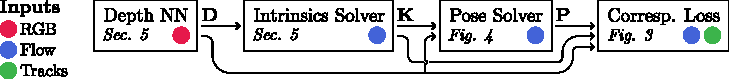
\includegraphics[width=\linewidth,]{figures/flowchart/fig_flowchart_pdf.pdf}
    \caption{\textbf{A FlowMap Forward Pass.}
    Given RGB frames (red), optical flow (blue) and point tracks (green), FlowMap computes dense depth $\depth$, camera poses $\pose$, and intrinsics $\ints$ in each forward pass. 
    We obtain depth via a CNN (\cref{sec:reparams}) and implement differentiable, feed-forward solvers for intrinsics and poses (\cref{sec:reparams}, Fig.\ref{fig:procrustes}).
    Colored dots indicate which block receives which inputs.
    FlowMap's only free parameters are the weights of a depth NN and a small correspondence confidence MLP.
    These parameters are optimized for each video separately by minimizing a camera-induced flow loss (Fig.~\ref{fig:loss}) via gradient descent, though fully feed-forward operation is possible.
    }
    \label{fig:flowchart}
    \vspace{-10pt}
\end{figure*}

\begin{figure*}[t]
    \centering
    \includegraphics[width=\linewidth]{figures/pdfs/point_clouds_small.pdf}
    \caption{\textbf{Point Clouds Reconstructed by FlowMap.} Unprojecting FlowMap depths using FlowMap's intrinsics and poses yields dense and consistent point clouds.}
    \label{fig:point_clouds}
    \vspace{-10pt}
\end{figure*}


\section{Results}
\label{sec:exp}

We benchmark FlowMap via the downstream task of 3D Gaussian reconstruction~\cite{kerbl20233d}.
This allows us to measure the quality of the camera parameters and geometry (depth maps) it outputs \emph{without having access to ground-truth scene geometry and camera parameters}.


\myparagraph{Baselines.}
We benchmark FlowMap against several baselines.
First, we evaluate against COLMAP~\cite{schonberger2016structure}, the state-of-the-art structure-from-motion (SfM) method.
Given a collection of images, COLMAP outputs per-image camera poses and intrinsics alongside a sparse 3D point cloud of the underlying scene.
3D Gaussian Splatting, which was designed around COLMAP's SfM outputs, is initialized using this point cloud.
Second, we evaluate against COLMAP multi-view stereo (MVS), which enhances COLMAP's output with a much denser 3D point cloud.
When initialized using this denser point cloud, 3D Gaussian Splatting produces slightly better results.
However, note that COLMAP MVS is rarely used in practice because it can be prohibitively time-consuming to run.
Third, we evaluate against DROID-SLAM, a neural SLAM system trained on a synthetic dataset of posed video trajectories.
Finally, we evaluate against NoPE-NeRF, an method that jointly optimizes a neural radiance field and unknown camera poses.
Note that unlike FlowMap and COLMAP, both DROID-SLAM and NoPE-NeRF require camera intrinsics as input.

\myparagraph{Datasets.}

We analyze FlowMap on four standard novel view synthesis datasets: MipNeRF-360~\cite{barron2021mipnerf}, Tanks \& Temples~\cite{Knapitsch2017tanks}, LLFF~\cite{mildenhall2019local}, and CO3D~\cite{reizenstein2021common}.
Because FlowMap runs on video sequences, we restrict these datasets to just the video-like sequences they provide.

\myparagraph{Methodology.}

We run FlowMap and the baselines using images that have been rescaled to a resolution of about 700,000 pixels.
We then optimize 3D Gaussian scenes for all methods except NoPE-NeRF, since it provides its own NeRF renderings.
We use 90\% of the available views for training and 10\% for testing.
During 3D Gaussian fitting, we follow the common~\cite{nerfstudio} practice of fine-tuning the initial camera poses and intrinsics.
Such refinement is beneficial because the camera poses produced by SfM algorithms like COLMAP are generally not pixel-perfect~\cite{park2023camp,lin2021barf}.
We use the 3D points provided by COLMAP, DROID-SLAM, and FlowMap as input to 3D Gaussian Splatting.
For FlowMap, we combine the output depth maps, poses, and intrinsics to yield one point per depth map pixel.

\subsection{Novel View Synthesis Results}

Tab.~\ref{tab:recon} reports rendering quality metrics (PSNR, SSIM, and LPIPS) on the held-out test views, and Fig.~\ref{fig:splat_comparison} shows qualitative results.
Qualitatively, FlowMap facilitates high-quality 3D reconstructions with sharp details.
Quantitatively, FlowMap performs slightly better than COLMAP SfM and significantly outperforms DROID-SLAM and NoPE-NeRF.
Only COLMAP MVS slightly exceeds FlowMap in terms of reconstruction quality.
As noted previously, COLMAP MVS is rarely used for 3D Gaussian Splatting, since it is very time-consuming to run on high-resolution images.

\subsection{Camera Parameter Estimation Results}

Since the datasets we use do not provide ground-truth camera parameters, they cannot be used to directly evaluate camera parameter estimates.
Instead, Tab.~\ref{tab:recon} reports the average trajectory error (ATE) of FlowMap, DROID-SLAM, and NoPe-NeRF with respect to COLMAP.
Since COLMAP's poses are not perfect~\cite{park2023camp}, this comparison is not to be understood as a benchmark, but rather as an indication of how close these methods' outputs are to COLMAP's state-of-the-art estimates.
We find that DROID-SLAM and FlowMap both recover poses that are close to COLMAP's, while NoPE-NeRF's estimated poses are far off.
When computing ATEs, we normalize all trajectories such that $\text{tr}(XX^T) = 1$, where $X$ is an $n$-by-3 matrix of camera positions.

Fig.~\ref{fig:trajectories} plots trajectories recovered by FlowMap against those recovered by COLMAP, showing that they are often nearly identical.
Fig.~\ref{fig:point_clouds} shows point clouds derived from FlowMap's estimated depth maps and camera parameters, illustrating that FlowMap recovers well-aligned scene geometry.

\subsection{Large-Scale Robustness Study}

\begin{figure*}[t!]
    \centering
    \includegraphics[width=\linewidth,]{figures/pdfs/colmap_study_hist.pdf}
    \vspace{-20pt}
    \caption{\textbf{Large-scale Robustness Study.}
    We run FlowMap and DROID-SLAM on 420 CO3D scenes across 10 categories and plot mean ATEs with respect to CO3D's COLMAP-generated pose metadata.
    We also re-run COLMAP on the same data.
    Compared to DROID-SLAM, which requires ground-truth intrinsics, FlowMap produces notably lower ATEs.
    FlowMap's ATE distribution is similar to one obtained by re-running COLMAP, with most ATEs falling under 0.005 in both cases.}
    \label{fig:colmap_study}
    \vspace{-5pt}
\end{figure*}


We study FlowMap's robustness by using it to estimate camera poses for 420 CO3D scenes from 10 categories.
We compare these trajectories to CO3D's pose annotations, which were computed using COLMAP.
Since the quality of CO3D's ground-truth trajectories varies between categories, we focus on categories that have been used to train novel view synthesis models~\cite{tewari2023diffusion,chan2023generative,wewer24latentsplat}, where pose accuracy is expected to be higher.
We find that FlowMap's mean ATE (0.0056) is lower than DROID-SLAM's (0.0082) and similar to the mean ATE obtained by re-running COLMAP and comparing the results to the provided poses (0.0038).
This demonstrates that FlowMap consistently estimates poses which are close to COLMAP's.
We note that COLMAP failed to estimate poses for 36 scenes, possibly because we ran it at a sparser frame rate to be consistent with our method or because the original annotations were generated using different COLMAP settings; we exclude COLMAP's failures from the above mean ATE.
See Fig.~\ref{fig:colmap_study} for distributions of ATE values with respect to CO3D's provided camera poses.
\vspace{-10pt}

	
	% % -------- Conclusion -------- %
	\section{Conclusion}

In this paper, we propose a pioneering approach to explore the source-free domain adaptation (SFDA) for video object detection (VOD). Specifically, we developed a novel SFDA method for a one-stage-based detector, YOLOV. The proposed STAR-MT technique significantly improves the performance of the video object detector in adverse image conditions without access to the target domain label or source domain data. Owing to its unsupervised nature, this work can be seamlessly applied to real-world scenarios requiring VOD models. The proposed method could serve as a baseline for future research in unsupervised domain adaptation for video object detection. 


	\clearpage
	
	\begin{center}
		\Large{\textbf{Efficient Transformer Encoders for Mask2Former-style models} \\ (Supplementary Material)}
		\vspace*{2em}
	\end{center}
	
	\renewcommand\thesection{\Alph{section}}
	\setcounter{section}{0}
	\setcounter{figure}{0}
	\renewcommand{\thefigure}{F\arabic{figure}}
	\setcounter{table}{0}
	\renewcommand{\thetable}{T\arabic{table}}
	
	% -------- Supp Material -------- %
	\section{Additional Experiments}

\paragraph{Impact of backbone size on Lite-M2F.} We apply {\ours} on Lite-M2F using various backbone sizes, including SWIN-Tiny (T), SWIN-Small (S), and SWIN-Base (B) architectures \cite{liu2021swin}. Lite-M2F is a specific variant based on Lite-DETR \cite{li2023lite}. We used the configuration named ``Lite-DETR H3L1-(6+1)$\times$1'' given its strong performance in detection relative to the computations required. However, we adjust this configuration to (5+1) when applying our approach to Lite-M2F. Further, we use their without the key-aware deformable attention  \cite{li2023lite} proposed in their paper. This adjustment is necessary because Lite-M2F actually has 6 encoder layers, and the original configuration might introduce an additional layer that isn't present in the model. Following this, we identify layers 2 to 5 as potential exits, followed by the last layer, layer 6 in the transformer encoder. We retain layer 6 and do not consider it as a feasible exit point as it leverages features from all scales provided by the backbone, making it essential to the model's functionality. As shown in \Tabref{tab:supp_result_backbones}, we observe that {\ours} effectively reduces computational cost while maintaining performance across Lite-M2F variants, which underscores the versatility and robustness of {\ours} across different model architectures and sizes.
%
\paragraph{Impact of target and loss settings for gating network training.} We investigate various target and loss settings during the training of the gating network. Specifically, we compare the approach detailed in the main paper, using one-hot target and cross-entropy loss (referred to as ``hard-CE'' in \Tabref{tab:tgt_loss}), with three alternative methods that do not involve setting a specific target exit for each image.

First, we consider using cross-entropy loss between the output of the utility function $\uF(\cdot)$ and the predicted logit passed through a softmax function (referred to as ``u-CE''), \ie, 
\[
\loss_\text{gating}=\sum_i^N\sum_{\Glayer}^{\NGlayer}\uF\superIdx(\Glayer)\ln [\text{softmax}(g_\Glayer\superIdx)]\,.
\]

Second, we apply a softmax function to the utility function $u(\Glayer)$ and use cross-entropy as the loss function (referred to as ``soft-CE''), \ie,
\[
\loss_\text{gating}=\sum_i^N\sum_{\Glayer}^{\NGlayer}\text{softmax}(\uF\superIdx(\Glayer))\ln [\text{softmax}(g_\Glayer\superIdx)]\,.
\]

Third, we apply a softmax function to the utility function, but use mean squared error (MSE) loss instead (referred to as ``soft-MSE''), \ie,
\[
\loss_\text{gating}=\sum_i^N\sum_{\Glayer}^{\NGlayer}\left[\text{softmax}(\uF\superIdx(\Glayer))-\text{softmax}(g_\Glayer\superIdx)\right]^2\,.
\]

The analysis in \Tabref{tab:tgt_loss} is conducted using the SWIN-T \cite{liu2021swin} backbone on the COCO dataset. We observe that ``hard-CE'' yields the most favorable results. As a result, we use this approach consistently in the main paper.

\begin{table}[!ht]

\begin{minipage}[!hb]{0.495\textwidth}
\centering
\caption{\textbf{Impact of backbone size on Lite-M2F.} Our Lite-{\ours} maintains the performance of Lite-M2F while reducing GFLOPs for different datasets and for different backbones.}
\resizebox{\columnwidth}{!}{
\begin{tabular}{llcccccccc}
\toprule
 && \multicolumn{3}{c}{\textbf{Performance} ($\uparrow$)} && \multicolumn{2}{c}{\textbf{GFLOPs} ($\downarrow$)} \\ \cline{3-5} \cline{7-8}
\multirow{-2}{*}{\textbf{Bakbone}} & \multirow{-2}{*}{\textbf{Model}} & \textbf{PQ} & \textbf{mIOU}$_p$ & \textbf{AP}$_p$ && \textbf{Total} & \textbf{Tx. Enc.} \\ 
\midrule

\multicolumn{8}{c}{\textbf{Dataset}: Cityscapes}\\
\hline
\multirow{2}{*}{\textbf{SWIN-T}}
& Lite-M2F \cite{li2023lite} & 62.29 & 79.43 & 36.57 && 428.71 & 172.00 \\
& Lite-{\ours} & 62.64 & 79.99 & 36.52 && 412.88 & 156.17 \\
\hline
\multirow{2}{*}{\textbf{SWIN-S}}
& Lite-M2F \cite{li2023lite} & 63.54 & 79.74 & 39.12 && 615.15 & 171.99 \\
& Lite-{\ours} & 63.32 & 80.21 & 37.91 && 588.82 & 145.66 \\


\hline
\multirow{2}{*}{\textbf{SWIN-B}} 
& Lite-M2F \cite{li2023lite} & 64.48 & 82.34 & 39.21 && 942.05 & 174.01 \\
& Lite-{\ours} & 64.66 & 81.40 & 39.52 && 921.15 & 153.11 \\

\hline
\multicolumn{8}{c}{\textbf{Dataset}: COCO}\\
\hline
\multirow{2}{*}{}\textbf{SWIN-T}
& Lite-M2F \cite{li2023lite} & 52.70 & 63.08 & 41.10 && 193.79 & 79.78 \\
& Lite-{\ours} & 52.84 & 63.23 & 42.18 && 178.43 & 64.42 \\
\hline
\multirow{2}{*}{\textbf{SWIN-S}} 
& Lite-M2F \cite{li2023lite} & 54.30 & 64.81 & 43.94 && 269.26 & 74.45 \\  
& Lite-{\ours} & 54.47 & 64.14  & 43.55 && 258.00 & 63.96 \\

\bottomrule
\end{tabular}}  
\label{tab:supp_result_backbones}
\end{minipage}
\hfill
\begin{minipage}[!hb]{0.495\textwidth}
\centering
\caption{\textbf{Impact of target and loss in gating network training.} We use ``hard-CE'' loss for training our gating network in the main paper. (Backbone: SWIN-T; Dataset: COCO)}
\resizebox{\columnwidth}{!}{
\begin{tabular}{lcccccccc}
\toprule
 & \multicolumn{3}{c}{\textbf{Performance} ($\uparrow$)} && \multicolumn{2}{c}{\textbf{GFLOPs} ($\downarrow$)} \\ \cline{2-4} \cline{6-7}
\multirow{-2}{*}{\textbf{Method}} & \textbf{PQ} & \textbf{mIOU}$_p$ & \textbf{AP}$_p$ && \textbf{Total} & \textbf{Tx. Enc.} \\ 
\midrule
\rowcolor{eccvblue!20}
hard-CE & 52.06 & 62.76 & 41.51 && 202.39 & 88.47 \\
u-CE & 52.16 & 62.58 & 41.57 && 207.49 & 94.06 \\
soft-CE & 51.64 & 62.75 & 40.88 && 202.08 & 87.85 \\
soft-MSE & 51.54 & 62.73 & 40.91 && 198.46 & 84.53 \\
\bottomrule
\end{tabular}}  
\label{tab:tgt_loss}
\end{minipage}

\end{table}

\section{Additional Qualitative Results}
We provide additional examples of predicted segmentation maps in \Figref{fig:supp_qual_result}.
\begin{figure}[!ht]
\begin{tcbraster}[enhanced,
    blank, 
    raster columns=3,
    raster equal height,
    ]
    \tcbincludegraphics[]{figures/qual_result_images/coco/exp9/000000176232.jpg}
    \tcbincludegraphics[]{figures/qual_result_images/coco/exp9/000000176232_m2f.jpg}
    \tcbincludegraphics[flip title={boxsep=0.75mm}]{figures/qual_result_images/coco/exp9/000000176232_ours.jpg}
    \vspace*{-2.5\baselineskip}
    %
    \tcbincludegraphics[]{figures/qual_result_images/coco/exp2/000000002149.jpg}
    \tcbincludegraphics[]{figures/qual_result_images/coco/exp2/000000002149_m2f.jpg}
    \tcbincludegraphics[flip title={boxsep=0.75mm}]{figures/qual_result_images/coco/exp2/000000002149_ours.jpg}
    \vspace*{-5\baselineskip}
    %
    \tcbincludegraphics[]{figures/qual_result_images/cityscapes/exp6/munster_000008_000019_leftImg8bit.png}
    \tcbincludegraphics[]{figures/qual_result_images/cityscapes/exp6/munster_000008_000019_leftImg8bit_m2f.png}
    \tcbincludegraphics[flip title={boxsep=0.75mm}]{figures/qual_result_images/cityscapes/exp6/munster_000008_000019_leftImg8bit_ours.png}
    \vspace*{-8\baselineskip}
    %
    \tcbincludegraphics[]{figures/qual_result_images/cityscapes/exp7/munster_000013_000019_leftImg8bit.png}
    \tcbincludegraphics[]{figures/qual_result_images/cityscapes/exp7/munster_000013_000019_leftImg8bit_m2f.png}
    \tcbincludegraphics[flip title={boxsep=0.75mm}]{figures/qual_result_images/cityscapes/exp7/munster_000013_000019_leftImg8bit_ours.png}
    \vspace*{-2\baselineskip}
   \end{tcbraster} 
    \caption{\textbf{Qualitative visualizations.} We provide additional examples of predicted segmentation maps from M2F \cite{cheng2021mask2former} (\textit{middle} column) and \ours (\textit{last} column). \textit{Top} two rows are from the COCO dataset, whereas \textit{bottom} two rows are from the Cityscapes dataset. Please zoom in for a clearer view of the details. (Backbone: SWIN-T)} 
    \label{fig:supp_qual_result}
\end{figure}
	
	%%%%%%%%% REFERENCES
	\FloatBarrier
	
	% ---- Bibliography ----
	%
	% BibTeX users should specify bibliography style 'splncs04'.
	% References will then be sorted and formatted in the correct style.
	%
	\bibliographystyle{splncs04}
	\bibliography{ref}
\end{document}